
\subsection{Experimental Evaluation}
We evaluated our method on several datasets containing PP quads of the form $\{v,n1,p,n2\}$.   The task is to predict if the  PP ($p,n2$) attaches to the verb $v$ or to the first noun $n1$. 


\subsubsection{Experimental Setup}\label{experimentalsetup}

\begin{table}[t]
%
\centering
%
\begin{tabular}{|l|l|l|}
\hline
{\bf DataSet} &  {\bf  \# Training quads} & {\bf \# Test quads} \\
\hline
\multicolumn{3}{|c|}{Labeled data} \\
    \hline
WSJ &  20,801 & 3,097 \\
NYTC & 0 & 293  \\
 WKP & 0 & 381  \\
      \hline
 \multicolumn{3}{|c|}{Unlabeled data} \\
      \hline
        %WSJ & - & - \\
         %NYTC & - & - \\
          WKP  & 100,000 & 4,473,072 \\
         
\hline
\end{tabular}
\caption{Training and test datasets used in our experiments. }
%\tom{What does "-" mean in this table?  If zero, let's use "0"}}
\label{tab:datasets}
\end{table}
     
    
     
\paragraph{Datasets}
Table~\ref{tab:datasets} shows the datasets used in our experiments. 
As labeled training data, we used the Wall Street Journal  (WSJ) dataset. For the unlabeled  training data, we extracted  PP quads from Wikipedia (WKP) and randomly selected $100,000$ which we found  to be a sufficient amount of unlabeled data.
The largest labeled test dataset is  WSJ
but it is also made up of a large fraction, of  ``of" PP quads, 30\% , which trivially attach to the noun, as already seen  in Figure \ref{fig:distribution}.
%and in general it is more comprehensive in the kind of prepositions it contains.
 The New York Times (NYTC) and Wikipedia (WKP) datasets are  smaller but contain fewer proportions  of ``of" PP quads, 15\%,  and 14\%, respectively. 
  %with a focus on  frequently used prepositions.
  Additionally, we applied our  model to over 4 million unlabeled 5-tuples from Wikipedia. We make this data available for download,  along with our manually labeled NYTC and WKP datasets.
For the WKP \& NYTC corpora,  each quad has a  preceding noun, $n0$, as context, resulting in PP 5-tuples of the form:  $\{n0,v,n1,p,n2\}$. The WSJ dataset was only available to us in the form of  PP quads with no other sentence information.

\begin{table}[t]
\centering
\begin{tabular}{|l|l|l|l|l|}
\hline
& PPAD& PPAD- &Coll-& Stan-\\
& & NB &ins& ford\\
\hline
WKP &  \bf{0.793} &	0.740&	0.727&	0.701\\
\hline
WKP  & \bf{0.759} &	0.698&	0.683&	0.652 \\
\textbackslash of  & & & & \\
\hline
NYTC & \bf{0.843}	& 0.792	&0.809	&0.679\\
\hline
NYTC& \bf{0.815}	& 0.754&	0.774&	0.621\\
\textbackslash of  & & & & \\
\hline
WSJ & \bf{0.843}&	0.816&	0.841& N\textbackslash A \\
\hline
WSJ & \bf{0.779}	& 0.741&	0.778&N\textbackslash A  \\
\textbackslash of  & & & & \\
\hline
\end{tabular}
 \caption{PPAD  vs. baselines.}
   \label{fig:resultmain}
\end{table}
    

\begin{figure}[t]
%
\centering
%
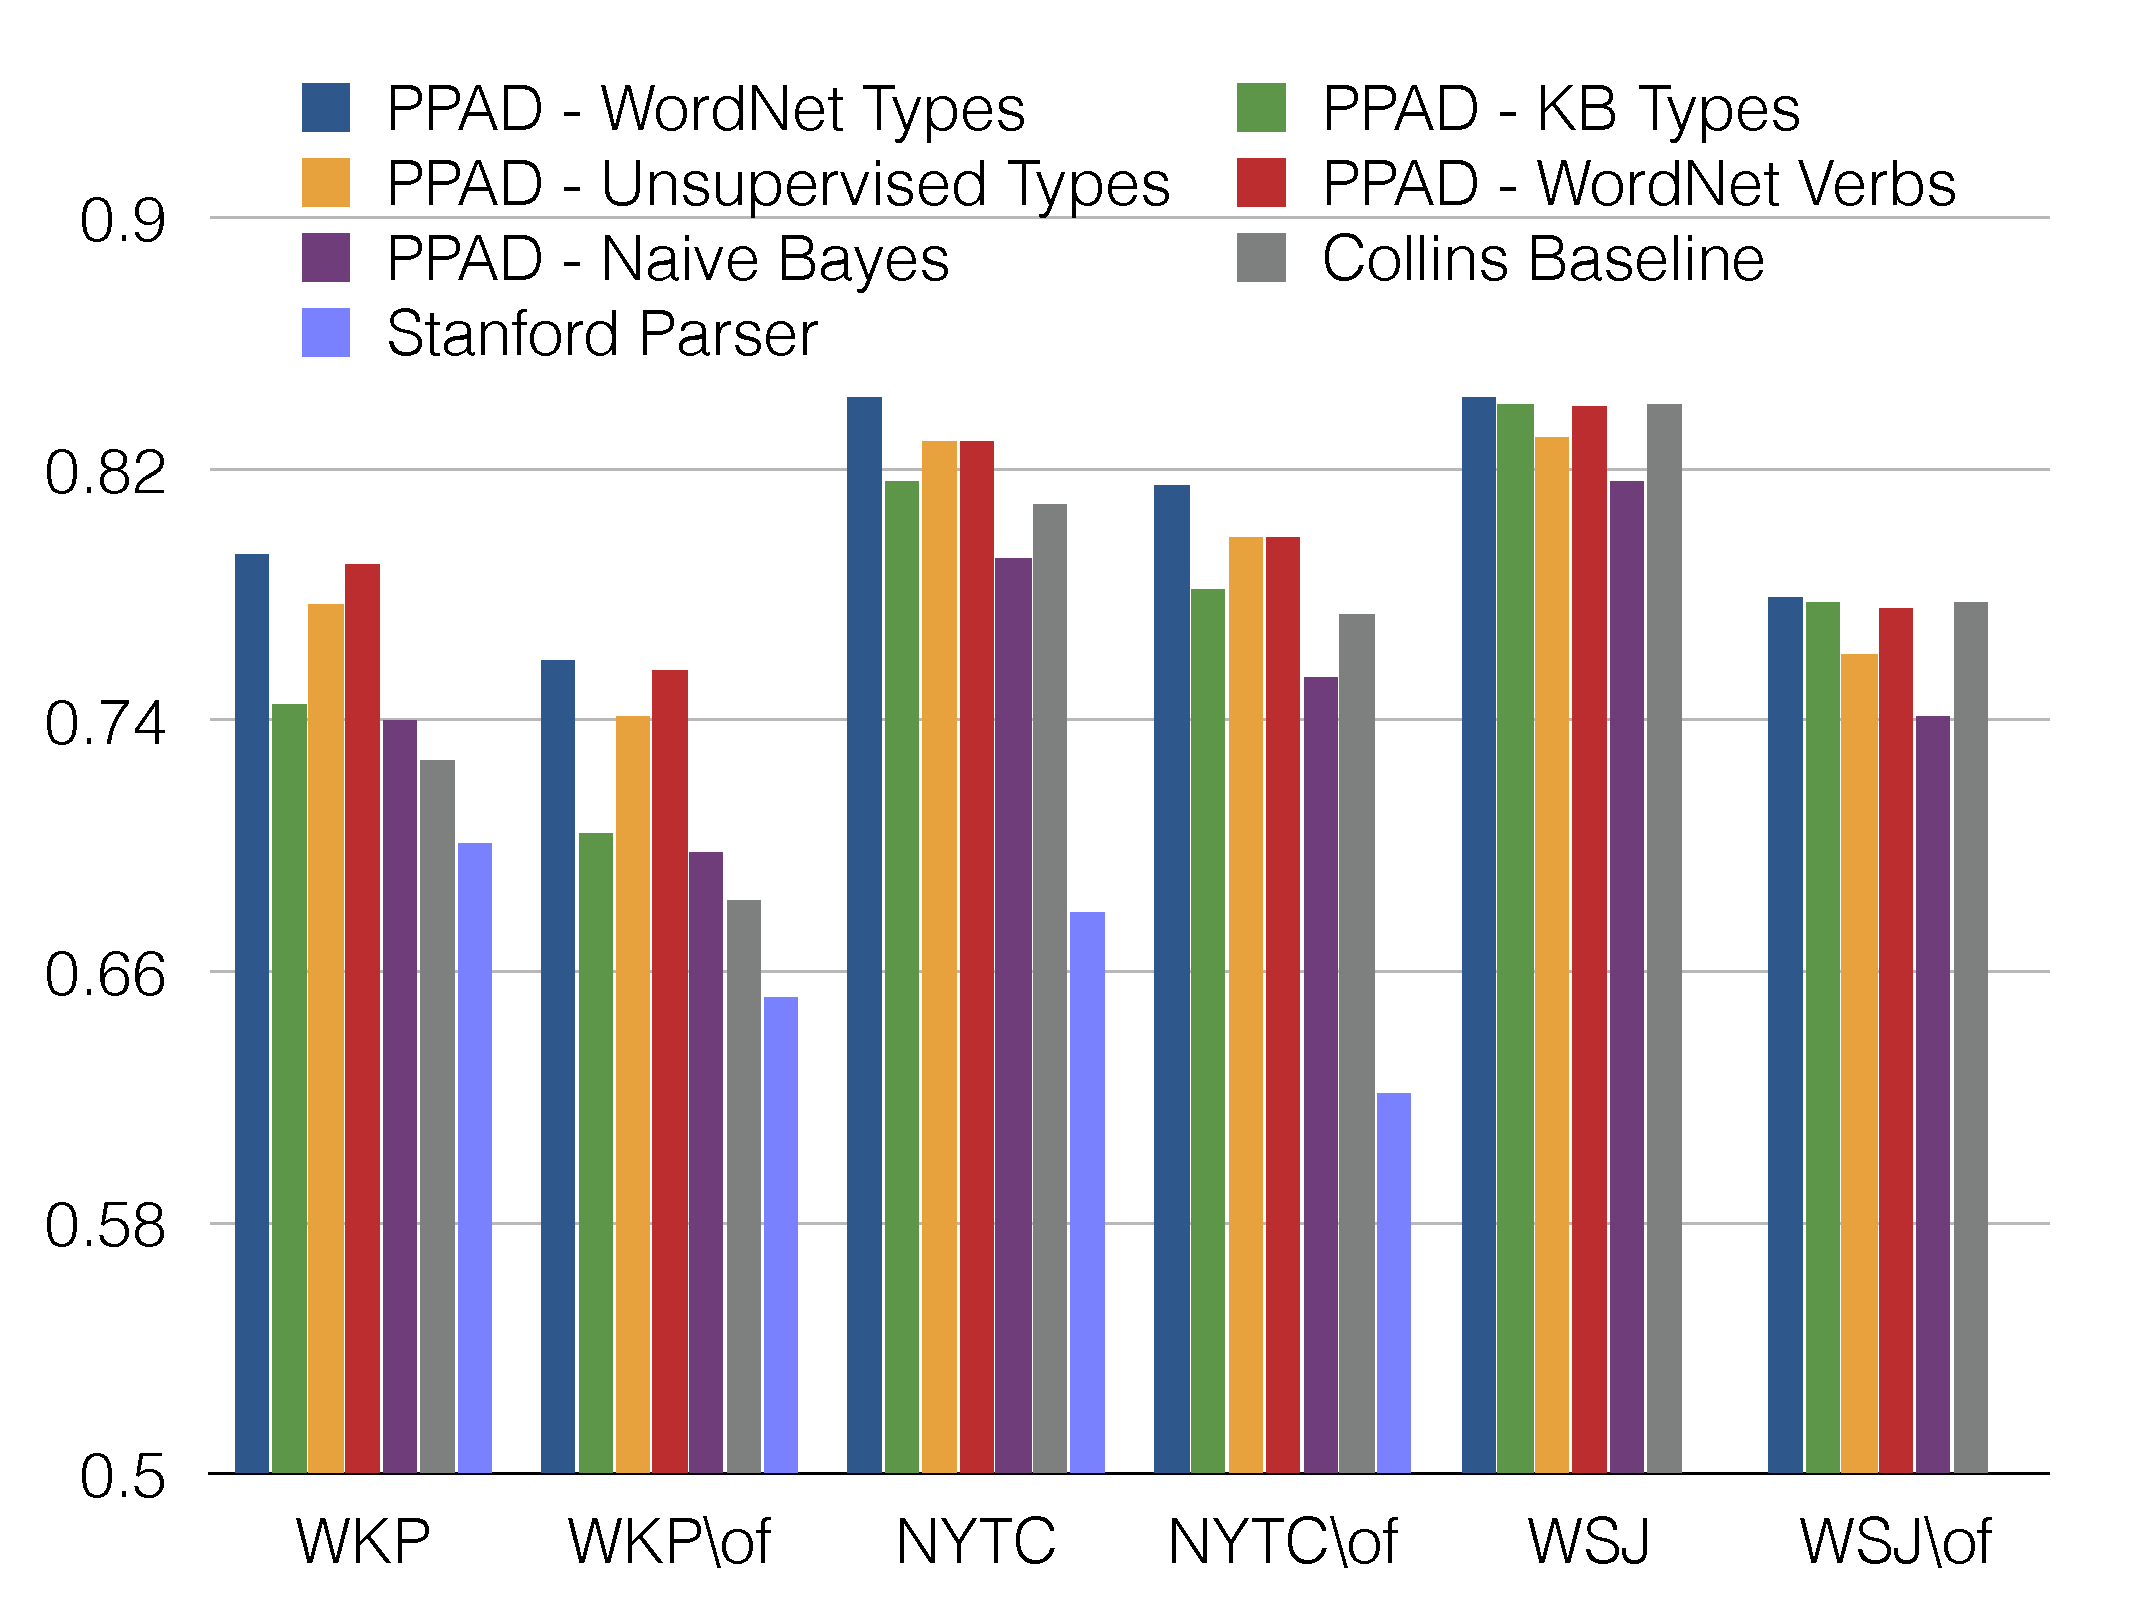
\includegraphics[width=1\columnwidth] {mainresults-2.pdf}
%
\vspace*{-1cm}
\caption{PPAD variations vs. baselines.}
%
\label{fig:resultmain2}
%
\end{figure}
    
   
    
 \paragraph{Methods Under Comparison} 
\textit{1) PPAD}  (Prepositional Phrase Attachment Disambiguator) is  our proposed method. It uses diverse types of semantic knowledge, a mixture of labeled and unlabeled data for training data, a logistic regression classifier, and expectation maximization (EM) for parameter estimation \textit{2) Collins} is the established baseline among PP attachment algorithms \cite{Collins95}.  \textit{3) Stanford Parser} is a state-of-the-art dependency parser, the 2014 online version. \textit{4) PPAD Naive Bayes(NB)}  is the same as PPAD but  uses a generative model,  as opposed to the discriminative model used in  PPAD.


 \subsubsection{PPAD vs. Baselines}
Comparison results of our method to the three baselines are shown in Table \ref{fig:resultmain}. For each dataset, we also show  results when the ``of" quads are removed, shown as ``WKP\textbackslash of'', ``NYTC\textbackslash of'', and ``WSJ\textbackslash of''.
 Our method yields  improvements over the baselines. Improvements are  especially significant on the datasets for which no labeled data was available  (NYTC and WKP). On  WKP, our method is 7\% and 9\% ahead of the Collins baseline and the Stanford parser, respectively.  On  NYTC, our method is 4\% and 6\% ahead of the Collins baseline and the Stanford parser, respectively. On WSJ, which is the source of the labeled data, our method  is not significantly  better than the Collins baseline. We could not evaluate the Stanford parser on the  WSJ dataset.  The parser requires well-formed sentences which we could not generate from the WSJ dataset as it was only available to us in the form of  PP quads with no other sentence information.  For the same reason,  we could not generate discourse features,$F7$, for the  WSJ PP quads.  For the  NYTC and WKP datasets, we generated well-formed short  sentences containing only the PP quad and the noun preceding it.  

 
 \subsubsection{Feature Analysis}
We found that features $F2$ and $F6$ did not improve performance, therefore we  excluded them from the final model, PPAD. This means that binary noun-noun relations were not useful when used permissively, feature $F2$, but when used selectively, feature $F1$, we found them to be useful. Our attempt at mapping prepositions to  verb definitions produced some noisy mappings, resulting in feature $F6$  producing mixed results.
To analyze the impact of the unlabeled data, we inspected the  features and their weights as produced by the PPAD model. From the unlabeled data, new  lexical features were discovered  that were not in the original labeled data.   Some sample  new features with high weights for verb attachments are: \textit{ (perform,song,for,*), %(*,independence,from,*),
(lose,*,by,*),  (buy,property,in,*)}. And for noun attachments: \textit{(*,conference,on,*), (obtain,degree,in,*), (abolish,taxes,on,*).} 
  %These newly discovered features could be the reason PPAD performs better than baselines on corpora for which no labeled data was available.


We evaluated several variations of PPAD, the results are shown in 
Figure \ref{fig:resultmain2}. For ``PPAD-WordNet Verbs",  we expanded the data by  replacing verbs in PP quads with synonymous WordNet verbs, ignoring verb senses.  This resulted in more instances of features F1, F8-10, \& F12. 

We also used  different types of noun categorizations: WordNet classes, semantic types from the NELL
knowledge base \cite{MitchellCHTBCMG15} and unsupervised types.  The KB types and the unsupervised types did not perform well, possibly due to the noise found in these categorizations.  WordNet classes showed the best results, hence they were used in  the final PPAD model for   features F3-4 \& F7.  In Section \ref{experimentalsetup}, PPAD corresponds to the best model.
  
     
     
 \subsubsection{Discussion: The F1 Score of Knowledge}
Why did we not  reach 100\% accuracy? Should relational knowledge not be providing a much bigger performance boost than we have seen in the results?
To answer these questions, we characterize our features in terms  precision and recall, and  F1 measure of their knowledge sources in Table \ref{fig:knowledgef1}. A low recall feature means that the feature does not fire on many examples, the feature's knowledge source suffers from low coverage.  A low precision feature means that when it fires, the feature could be incorrect, the feature's knowledge source contains a lot of errors. 
  

\begin{table*}[ht]
%
\centering
%
\begin{tabular}{|l|l|l|l|}
\hline 
\textbf{Feature Type} & \bf{Precision}  & \bf{Recall} & \bf{F1}\\
\hline
Noun-Noun Binary Relations (F1-2) &$low$ & $high$ &  $low$\\
Noun Semantic Categories (F3-4) & $high$ & $high$& \bf{high}\\
Verb Role Fillers (F5) & $high$ & $low$ & $low$ \\
Preposition Definitions (F6) & $low$ & $low$  &$low$ \\
Discourse Features (F7) & $high$ & $low$ & \bf{high} \\
Lexical Features (F8-15) & $high$ & $high$ & \bf{high} \\
\hline
\end{tabular}
\caption{An approximate characterization of feature knowledge sources in terms of precision/recall/F1}
 \label{fig:knowledgef1}
\end{table*}  
  
From Table \ref{fig:knowledgef1}, the  noun-noun binary relation features $(F1-2)$ have low precision, but high recall.
This is because the SVO data, extracted   from the ClueWeb09 corpus, that we used as  our  relational knowledge source is very noisy but it is high coverage. The low precision of the SVO data  causes these features to be detrimental to performance.  Notice that when we used a filtered version of the data, in feature $F2$, the data was no longer detrimental to performance. However, the $F2$ feature is low recall, and therefore it's impact on performance is also limited. The noun semantic category features $(F3-4)$ have high recall and precision, hence it to be expected that their impact on performance is significant. The verb role filler features  $(F5)$, obtained from VerbNet  have high precision but low recall, hence their marginal impact  on performance is also to be expected. The preposition definition features $(F6)$  poor precision made them unusable.  The discourse features $(F7)$  are based  noun semantic types and lexical features ($F8-15$),  both of which have high recall and precision, hence they useful impact on performance. 

In summary, low precision in knowledge is detrimental to performance. In order for knowledge to make even more significant contributions to language understanding, high precision, high recall knowledge sources are required for all features types. Success in ongoing efforts in knowledge base construction projects, will make performance of our algorithm better.  

\subsubsection{Application to Ternary Relations} \label{ternary}
Through the application of ternary relation extraction,  we further tested PPAD's PP disambiguation accuracy and  illustrated its usefulness for knowledge base population.
%In particular,  we studied accuracy on PP-attachments that express tenary relations by extending binary relations with one more argument.
Recall that a PP  5-tuple of the form $\{n0, v, n1, p, n2\}$, whose enclosed PP   attaches to the verb $v$,  denotes a ternary relation with  arguments \textit{n0, n1, \& n2}.
Therefore, we can extract a ternary relation from every 5-tuple for which our method predicts a verb attachment.   If we have a mapping between verbs and binary relations from a knowledge base (KB), we can extend KB relations to ternary relations by augmenting the KB relations with a third argument $n2$. 


\begin{table*}[ht]
%
\centering
%

\begin{tabular}{lp{1.4cm}lp{5.8cm}}
\hline
{\bf  Relation} &  {\bf  Prep. } & {\bf  Attachment accuracy}   &{\bf Example(s) } \\
\hline
acquired
%\newline purchased \newline bought
& from  & \textbf{99.97}  
& BNY Mellon	\textit{acquired}	Insight 	\textit{from}	Lloyds.\\
% \newline  \small{U.S.	\textit{bought}	Alaska	\textit{from}		Russian Rmpire.} \\
%\newline \small{Boeing	\textit{bought}	Jeppesen	\textit{from}	Tribune Company.}
%\newline  \small{Carolina Panthers	\textit{acquired}	Mccown	\textit{from}	Dolphins.}\\
\hline
hasSpouse & in  & \textbf{91.54} & David \textit{married}	Victoria	\textit{in}	Ireland.  \\
%\newline \small{Potts	\textit{married}	
%Alden Brown	\textit{in}	civil ceremony.}
%\newline \small{Henry Tate	\textit{married} Jane Wignall	\textit{in}	1885.}\\
\hline
	worksFor  & as & \textbf{99.98} & 
%	\small{Hillyer	\textit{joined} Boston Symphony Orchestra \textit{as}	violinist.} \newline
Shubert	\textit{joined}	CNN	\textit{as}	reporter. \\
		\hline
playsInstrument   & with & \textbf{98.40}  & Kushner	\textit{played}	 guitar	\textit{with}	rock band Weezer. \\
%\newline \small{Frehley	\textit{played}	lead guitar	\textit{with}	Chad Kroeger.} \\
\hline
%	musicianpla- \newline ysinstrument & played & for & \textbf{81.71}  & \small{Forminoya	\textit{played}	violin	\textit{for}	Eleanor Roosevelt.} \newline \small{Chilton Price	\textit{played}	violin	\textit{for}	Louisville Orchestra.}  \\
%     \hline
\end{tabular}
  \caption{Binary relations extended to ternary relations by mapping to verb-preposition pairs in PP 5-
tuples. PPAD predicted verb attachments with accuracy \textgreater 90\% in all relations.}
   \label{tab:tenary}
  \end{table*}
      
 % and the relation is expressed by the verb $v$.
We considered four KB binary relations and their instances such as $worksFor(Tim Cook, Apple)$, from the NELL KB. We then took the collection of 4 million 5-tuples  that we extracted from Wikipedia. We mapped verbs in 5-tuples to KB relations, based on  significant overlaps in the instances of the KB relations, noun pairs such as $(Tim Cook, Apple)$ with the  $n0,n1$ pairs in the Wikipedia PP 5-tuple collection. We found that, for example,  instances of the noun-noun KB relation ``worksFor" match $n0,n1$ pairs in tuples where  $v= joined$ and  $p=as$ , with  $n2$ referring  to the job title.  Other binary relations extended are: ``hasSpouse" extended by ``in" with wedding location, ``acquired" extended by ``from" with the  seller of the company being acquired.  Examples are  shown in Table \ref{tab:tenary}. 
In all these mappings, the proportion of verb attachments in the corresponding PP quads is significantly  high ( $ > 90\%$). PPAD is overwhelming  making the right attachment decisions in this setting.

Efforts in temporal and spatial relation extraction have shown that higher N-ary relation extraction is challenging.  Since prepositions specify details that transform binary relations to higher N-ary relations, our method can be used to read information that can augment  binary relations already in KBs. As future work, we would like to incorporate our method into a pipeline for reading beyond binary relations. One possible direction is to read details about the \textit{where,why, who} of events and relations, effectively moving from extracting only binary relations to reading at a more general level.


\subsubsection{Labeled Ternary Arguments}
In the above experiment, we studied the case of extending existing KB relations to ternary relations
with a third argument. However, we did not have any semantic information about the role of the third arguments. In this section, we study a different case, the case when we want to label the role of the third argument. For example, for the acquisition instance of ``BNY Mellon acquired Insight from Lloyds",  we want to predict that the label of ``Lloyds" is the ``Source",  indicating the source company of acquisition.  As another example, consider the buy instance `Bailey	bought	earrings	for	Josie",  we want to predict that the label of ``Josie" is ``Beneficiary", indicating the beneficiary of the earrings bought. 

To obtain labels for third arguments, we make use of VerbNet \cite{KipperKRP08}. VerbNet provides, for each verb, frames of the different use cases of the verb. Here we consider only  verb uses  that make use of prepositions. In VerbNet, these frames are described using a  label of ``primary=NP V NP PP.label" where the ``label" is the role of the third arguments following the prepositional phrase. One example is ``primary=NP V NP PP.instrument", each such frame is accompanied by an example sentence. In this case the example is: ``Paula hit the ball  with a stick", where the ``stick" takes the role of the instrument. Notice  that a given  verb and preposition combination does not necessary invoke a given label. For example in ``Paula hit the ball with joy", ``joy" does not play the role of the instrument. Therefore,  we learn introduce further constraints. We learn these constraints from the collection of 4 million 5-tuples  that we extracted from Wikipedia as explained in Section \ref{experimentalsetup}. In particular, we  replace mentions of entities with their NELL and WordNet semantic types. Using this approach, we generate templates of the form:
  \begin{table}[h]
  %
 \centering
  %
     \begin{tabular}{ll}
       \hline
\textless np\_v\_np\_pp.LABEL \textgreater \textless verb\textgreater \textless typeofArg1\textgreater \textless preposition \textgreater \textless typeofArg2\textgreater \\
            \hline
     \end{tabular}
       \label{tab:ternarylabels}
     \end{table}
    

We worked with five labels from VerbNet: 
np\_v\_np\_pp.beneficiary, np\_v\_np\_pp.instrument,\\ np\_v\_np\_pp.asset,
 np\_v\_np\_pp.source, and  np\_v\_np\_pp.topic. 
 Examples of learned templates for each of the five labels are as shown below in Table \ref{tab:ternarylabelsTemplates}.
 \begin{table}[h]
  %
 \centering
  %
     \begin{tabular}{ll}
       \hline
       
\textless np\_v\_np\_pp.beneficiary \textgreater \textless buy\textgreater \textless jewelry\textgreater \textless for \textgreater  \textless person\textgreater \\
 
\textless np\_v\_np\_pp.instrument \textgreater \textless shoot\textgreater \textless person\textgreater \textless with \textgreater \textless weapon\textgreater \\

\textless np\_v\_np\_pp.asset \textgreater \textless sell\textgreater \textless company\textgreater \textless for \textgreater \textless amount\textgreater \\

\textless np\_v\_np\_pp.source \textgreater \textless buy\textgreater \textless organization\textgreater \textless from \textgreater \textless organization\textgreater \\

\textless np\_v\_np\_pp.topic \textgreater \textless ask\textgreater \textless person\textgreater \textless for \textgreater \textless advice\textgreater \\
  
  \textless np\_v\_np\_pp.topic \textgreater \textless ask\textgreater \textless person\textgreater \textless for \textgreater \textless divorce\textgreater \\
            \hline
     \end{tabular}
     \caption{Examples of learned templates for labeled ternary relations}
       \label{tab:ternarylabelsTemplates}
     \end{table}
     
Table \ref{tab:ternarylabels}  shows sample instances of the different learned  templates for labeled ternary arguments.
We randomly sampled 100 such instances evaluated them for accuracy, we found a sampling accuracy of 88\%.


  \begin{table}[h]
  %
 \centering
  %
     \begin{tabular}{ll}
        \hline
        Ternary argument label &  Instance \\
       \hline
 np\_v\_np\_pp.beneficiary &	danai udomchoke	won	gold medal	for	thailand	\\
%np\_v\_np\_pp.beneficiary	& ian epton	won	gold medal	for	south africa	 \\
np\_v\_np\_pp.beneficiary &	alton	cooked	breakfast	for	crew	 \\
np\_v\_np\_pp.beneficiary & 	boys	cooked	cakes	for	girls	 \\
%np\_v\_np\_pp.beneficiary & 	mama	buys	piggy bank	for	cubs	 \\
np\_v\_np\_pp.beneficiary &	bailey	buys	earrings	for	josie	 \\
%np\_v\_np\_pp.beneficiary &	resources	buys	merchandise	for	attendees	 \\
%np\_v\_np\_pp.beneficiary &	duncan busby busby	won	gold medals	for	england	 \\
np\_v\_np\_pp.beneficiary &	jim	buys	bracelet	for	kathy	 \\
np\_v\_np\_pp.beneficiary &	leonard	buys	engagement ring	for	michelle	 \\
%np\_v\_np\_pp.beneficiary &	characters	buys	wine coolers	for	teenagers	 \\
np\_v\_np\_pp.beneficiary &	headmaster	bought	goggles	for	children	 \\
%np\_v\_np\_pp.beneficiary &	mayor bertrand-geslin	bought	collection	for	town	 \\
np\_v\_np\_pp.instrument &	lord edward thynne	shot	golden eagle	with	rifle	 \\
%np\_v\_np\_pp.instrument &	wahoo	opened	fire	with	mm guns	 \\
np\_v\_np\_pp.instrument &	mohawks	opened	fire	with	gunshots	 \\
%np\_v\_np\_pp.instrument &	portuguese garrison	opened	fire	with	artillery	 \\
np\_v\_np\_pp.instrument &	unidentified militants	opened	fire	with	grenade launcher	 \\
np\_v\_np\_pp.instrument &	jarvis	opened	fire	with	5-inch guns	 \\
np\_v\_np\_pp.instrument &	prince	stabs	vizier	with	dagger	 \\
np\_v\_np\_pp.instrument &	isaac van scoy	killed	british soldier	with	pitchfork	 \\
np\_v\_np\_pp.instrument &	ambush positions	opened	fire	with	mortars	 \\
np\_v\_np\_pp.instrument &	tamalika karmakar	killed	rebecca	with	knife	 \\
%np\_v\_np\_pp.instrument &	u-185	opened	fire	with	aa guns	 \\
np\_v\_np\_pp.source & telugu film homam	drew	inspiration	from	martin scorsese \\
np\_v\_np\_pp.source&	john coltrane	received	call	from	davis	 \\
np\_v\_np\_pp.source&	kenneth o'keefe	received	letter	from	state department	 \\
np\_v\_np\_pp.source&	tony	receives	letter	from	mandy	 \\
%np\_v\_np\_pp.source&	daughter	bought	tie	from	school	 \\
np\_v\_np\_pp.source&	peter	receives	call	from	claire	 \\
np\_v\_np\_pp.source&	huppertz	drew	inspiration	from	richard wagner	 \\
np\_v\_np\_pp.source&	fiz	receives	call	from	alan hoyle	 \\
np\_v\_np\_pp.source&	elbaz	drew	inspiration	from	bruce willis	 \\
np\_v\_np\_pp.source&	smolensky	bought	company	from	wheeler	 \\
n %p\_v\_np\_pp.topic&	marston	asks	marshall	for	help	 \\
%np\_v\_np\_pp.topic&	dead woman	asked	jack harper	for	help	 \\
np\_v\_np\_pp.topic&	wittenberg	asked	jan kazimierz	for	permission	 \\
np\_v\_np\_pp.topic&	brando	asked	john gielgud	for	advice	 \\
np\_v\_np\_pp.topic&	lutician delegates	asked	conrad	for	help	 \\
%np\_v\_np\_pp.topic&	doggett	asks	hayes	for	help	 \\
%np\_v\_np\_pp.topic&	marshall	asks	barney	for	advice	 \\
np\_v\_np\_pp.topic&	logan	asked	scott	for	help	 \\
%np\_v\_np\_pp.topic&	insult comic dog	asks	lopez	for	permission	 \\
np\_v\_np\_pp.topic&	philadelphia quakers	asked	nhl	for	permission	 \\
%np\_v\_np\_pp.topic&	hume	asked	john paul ii	for	permission	 \\
%np\_v\_np\_pp.topic&	hallman	asked	ncaa	for	permission	 \\
%np\_v\_np\_pp.topic&	countless times	asked	user	for	help	 \\
np\_v\_np\_pp.topic& steven	asks	frank	for	advice	 \\
%np\_v\_np\_pp.topic&	clerk	asks	peter	for	help	 \\
%np\_v\_np\_pp.topic&	commander wheeler	asks	hatfield	for	permission	 \\
%np\_v\_np\_pp.topic&	linden	asks	holder	for	help	 \\
np\_v\_np\_pp.topic&	rowe	asked	jackson	for	divorce	 \\
            \hline
     \end{tabular}
     \caption{Sample instances of    templates learned for labeled ternary arguments. For each instance, the label applies
     to the last argument.}
       \label{tab:ternarylabels}
     \end{table}

\subsection{Prepositional Phrase Attachment Ambiguity  Summary}
We have presented a knowledge-intensive  approach to prepositional phrase (PP) attachment disambiguation, which is  a type of syntactic ambiguity. Our method incorporates  knowledge about verbs, nouns, discourse, and noun-noun binary relations.   We trained a model using labeled data and unlabeled data, making use of expectation maximization for  parameter estimation.
% Future work includes using our method in  higher-nary relation extraction.
Our method can be seen as an example of tapping into a positive feedback loop for machine reading, which has only become possible in recent years due to the progress made by  information extraction and knowledge base construction techniques.


 
 
